\documentclass[10pt,aspectratio=169]{beamer}

\usepackage{graphicx,amsmath,amssymb,tikz,psfrag,pgfgantt,booktabs,array}
\usepackage{pgfplots}
\pgfplotsset{compat=1.16}
\usepgfplotslibrary{groupplots}
\usepackage[utf8]{inputenc}
\usepackage[T1]{fontenc}
\usepackage{lmodern}
\usetikzlibrary{positioning,fit,arrows.meta,backgrounds}

\usefonttheme[onlymath]{serif}

\input defs.tex

%% formatting

\mode<presentation>
{
\usetheme{default}
}
\setbeamertemplate{navigation symbols}{}
\usecolortheme[rgb={0.13,0.28,0.59}]{structure}
\setbeamertemplate{itemize subitem}{--}
\setbeamertemplate{frametitle} {
	\begin{flushleft}
	  {\large\bf \insertframetitle}
	\end{flushleft}
}

\newcommand\footlineon{
  \setbeamertemplate{footline} {
    \begin{beamercolorbox}[ht=2.5ex,dp=1.125ex,leftskip=.8cm,rightskip=.6cm]{structure}
      \footnotesize \insertshorttitle
      \hfill
      {\insertsectionnumber.\insertframenumber}
    \end{beamercolorbox}
    \vskip 0.45cm
  }
}
\footlineon

%% ---- OPCION A: lamina azul numerada (desactivada por limite de 15 laminas) ----
% \AtBeginSection[]{
%   \begin{frame}[plain]
%     \vspace*{-1.5em}
%     \begin{center}
%       {\Large\color{structure} \insertsectionnumber.~\insertsection}
%     \end{center}
%   \end{frame}
%   \setcounter{framenumber}{0}
% }

%% ---- solo reinicia la numeracion, sin lamina divisoria ----
\AtBeginSection[]{\setcounter{framenumber}{0}}

% % ---- OPCION B: indice destacado ----
% \AtBeginSection[]{
%   \begin{frame}[plain]{Outline}
%     \tableofcontents[currentsection]
%   \end{frame}
%   \setcounter{framenumber}{0}
% }

%% begin presentation

\title[Clustering y anomalías en estrellas periódicas de ALeRCE]{Clustering y anomalías en curvas de luz de estrellas periódicas}

\author[Grupo 5B]{Gabriel Fonseca \qquad Tomás Olave}

\date{}

\begin{document}

\begin{frame}[plain]
\vspace*{-1em}

% --- fila de logos ---
\hfill
\includegraphics[height=1.8cm]{figures/departments/fcfm_escudo_azul_png.png}

\vspace{1.2em}

% --- título y datos ---
\begin{center}

{\normalsize\color{gray}
Presentación Preliminar de Proyecto --- EL4106 Inteligencia Computacional}\\[1em]

{\Large\color{structure}
Clustering y anomalías en curvas de luz\\[0.25em]
de estrellas periódicas}\\[1.5em]

{\normalsize
Gabriel Fonseca \quad Tomás Olave}\\[0.4em]

{\footnotesize\color{gray}
Grupo 5B}\\[1.3em]

{\footnotesize
Profesor: Pablo Estévez \\[0.3em]
Profesor Auxiliar: Pablo Cornejo \\[0.3em]
Ayudante: Christian Díaz Guerra \\[0.6em]
Octubre 2026}

\end{center}

\end{frame}


% ---------- 1. Explicacion del tema: problema, motivacion, objetivos y estado del arte ----------
% ============================================================
% Seccion: Explicacion del tema
% Problema, motivacion, objetivos y estado del arte
% ============================================================
\section{Tema de estudio}

% ============================================================
\begin{frame}
\frametitle{Problema y motivación}
\vspace{-0.6em}
{\small
\begin{itemize}\itemsep=3pt
\item \textbf{Curva de luz}: brillo de una estrella en el tiempo. En una estrella periódica
  se repite cada cierto \textbf{período}
\item \textbf{ALeRCE} procesa las alertas del survey ZTF y resume cada curva en
  \textbf{178 features}: período, amplitud, color, etc.
\item \textbf{Problema}: 178 números por estrella no se pueden inspeccionar a ojo. Se necesita un
  espacio de pocas dimensiones donde aparezcan grupos y se distingan los objetos raros
\item \textbf{Motivación}: los surveys generan más alertas de las que se pueden revisar a mano,
  y los objetos que no calzan con ninguna clase conocida son los de mayor interés
\end{itemize}
}
\vspace{-0.3em}
\begin{center}
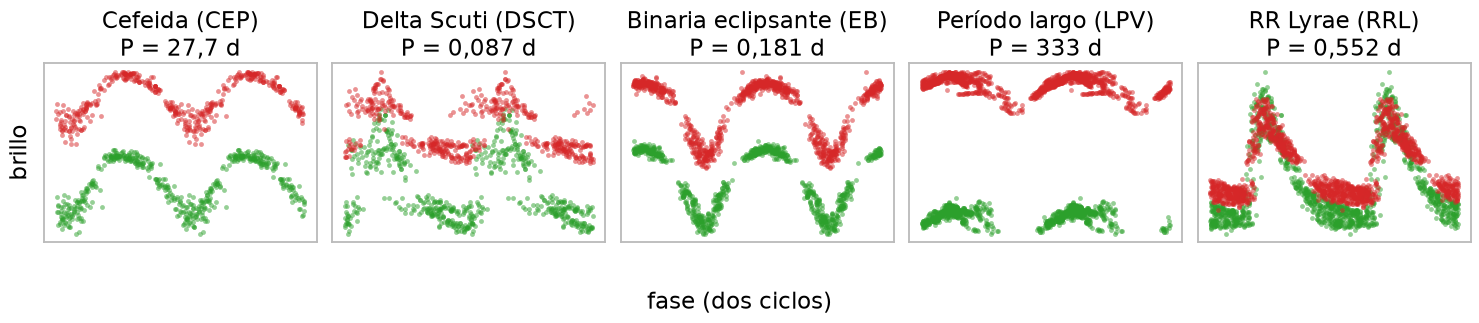
\includegraphics[width=0.86\textwidth]{figures/clases_curvas.png}\\[-0.2em]
{\scriptsize Las cinco clases del proyecto: curva plegada de un objeto típico de cada una
\quad$\cdot$\quad
\textcolor{green!55!black}{$\blacksquare$} banda g \quad \textcolor{red!80!black}{$\blacksquare$} banda r}
\end{center}
\end{frame}

% ============================================================
\begin{frame}
\frametitle{Objetivos y estado del arte}
\vspace{-0.5em}
\begin{columns}[T]
\begin{column}{0.50\textwidth}
{\small \textbf{Objetivo general}}
\vspace{0.2em}

{\footnotesize Agrupar estrellas variables periódicas de ALeRCE--ZTF en el espacio latente de un
autoencoder, y analizar los grupos y los posibles outliers a partir de sus curvas de luz.}

\vspace{0.7em}
{\small \textbf{Etapas del proyecto}}
\vspace{0.1em}
{\footnotesize
\begin{enumerate}\itemsep=3.5pt
\item Exploración preliminar de los datos con visualizaciones (UMAP, t-SNE, \emph{corner plots})
\item Visualización con autoencoders: cuello de botella de 2 dimensiones o más
\item Clustering con mezcla de gaussianas (GMM) y Multi-Class Deep SVDD sobre el cuello de botella
\item Visualización de las curvas de luz de los clusters y análisis de outliers
\end{enumerate}
}
\end{column}

\begin{column}{0.47\textwidth}
{\small \textbf{Estado del arte}}
\vspace{0.1em}
{\footnotesize
\begin{itemize}\itemsep=4.5pt
\item \textbf{ALeRCE} {\color{gray}(Förster et al.\ 2021)}: broker que clasifica alertas de ZTF.
  Su clasificador de curvas de luz usa las features de este proyecto
  {\color{gray}(Sánchez-Sáez et al.\ 2021)}
\item \textbf{DAGMM} {\color{gray}(Zong et al.\ 2018)}: autoencoder más mezcla de gaussianas en el
  espacio latente. Una verosimilitud baja marca la anomalía
\item \textbf{Deep SVDD} {\color{gray}(Ruff et al.\ 2018)}: un encoder que contrae los datos
  normales alrededor de un centro
\item \textbf{Multi-Class Deep SVDD} {\color{gray}(Pérez-Carrasco et al.\ 2023)}: un centro por
  clase conocida. Es el detector de anomalías de ALeRCE
\end{itemize}
}
\end{column}
\end{columns}
\end{frame}


% ---------- 2. Trabajo realizado y metodologia ----------
% ============================================================
% Seccion: Trabajo realizado y metodologia
% Etapa 1 (exploracion), decisiones de preprocesamiento y arquitectura
% Figuras: figures/umap_features.png, importancia_nan.png, escala_latente.png
% ============================================================
\section{Trabajo realizado y metodología}

% ============================================================
\begin{frame}
\frametitle{Etapa 1: datos y exploración}
\vspace{-0.5em}
\begin{columns}[T]
\begin{column}{0.40\textwidth}
{\small
\begin{itemize}\itemsep=4pt
\item \textbf{8.419 estrellas} con features y clase, de 9.829 etiquetadas
\item \textbf{5 clases desbalanceadas}\\[0.25em]
  {\footnotesize EB 2.689 \quad RRL 2.652 \quad LPV 1.374\\[0.1em] CEP 1.172 \quad DSCT 532}
\item \textbf{178 features} por objeto, 166 con datos faltantes
\item \textbf{Sin preprocesar} no aparece estructura: una sola feature domina las distancias
\item \textbf{Preprocesamiento aplicado}: descarte de 20 features, logaritmos, recorte de
  valores extremos, imputación con la mediana y z-score
\end{itemize}
}
\end{column}

\begin{column}{0.58\textwidth}
\centering
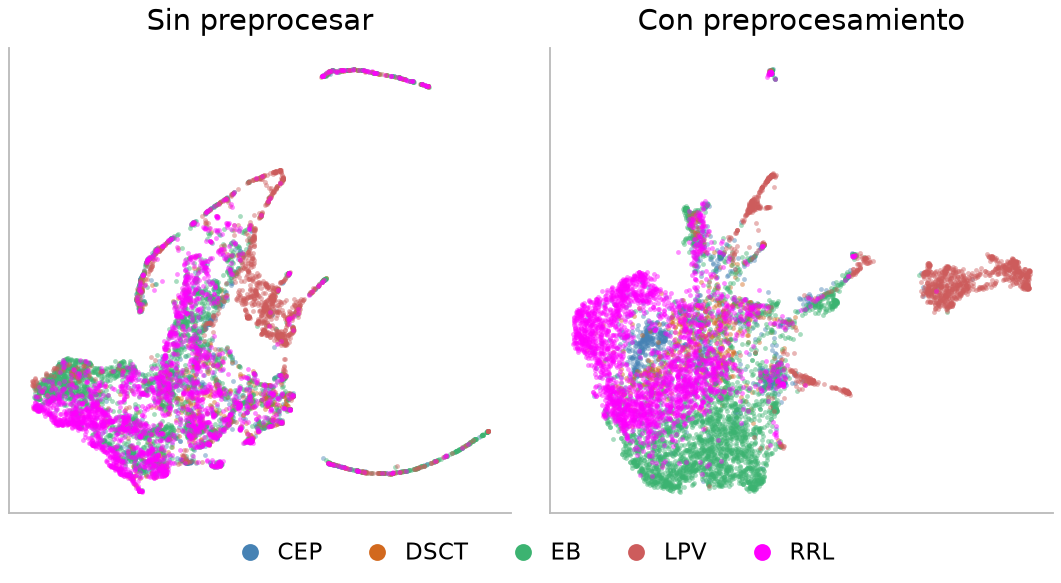
\includegraphics[width=\textwidth]{figures/umap_features.png}\\[0.1em]
{\scriptsize UMAP (\texttt{n\_neighbors} = 20) de las features de los 8.419 objetos.\\
Con el preprocesamiento LPV se separa y aparecen zonas por clase}
\end{column}
\end{columns}
\end{frame}

% ============================================================
\begin{frame}
\frametitle{Decisión 1: features, transformaciones y recorte}
\vspace{-0.5em}
\begin{columns}[T]
\begin{column}{0.53\textwidth}
{\small
\begin{itemize}\itemsep=3pt
\item \textbf{Se descartan 20 de 178}: 14 de no-detecciones previas a la primera alerta y 6
  colores WISE. Su dato faltante no es física de la estrella
\item \textbf{Verificación}: un random forest obtiene el mismo F1 macro con 158 features que
  con 178 (0,92)
\item \textbf{Logaritmo}: $\log_{10}$ a los tres períodos, que van de horas a cientos de días, y
  $\log(1+x)$ a 20 features positivas de cola larga
\item \textbf{Recorte de valores extremos}: cada feature se limita al rango entre sus
  percentiles 1 y 99 de train. Lo que queda fuera se reemplaza por el límite, sin eliminar
  objetos. Afecta al 1,8\,\% de los valores
\item \textbf{Después}: imputación con la mediana y z-score
\end{itemize}
}
\end{column}

\begin{column}{0.45\textwidth}
\centering
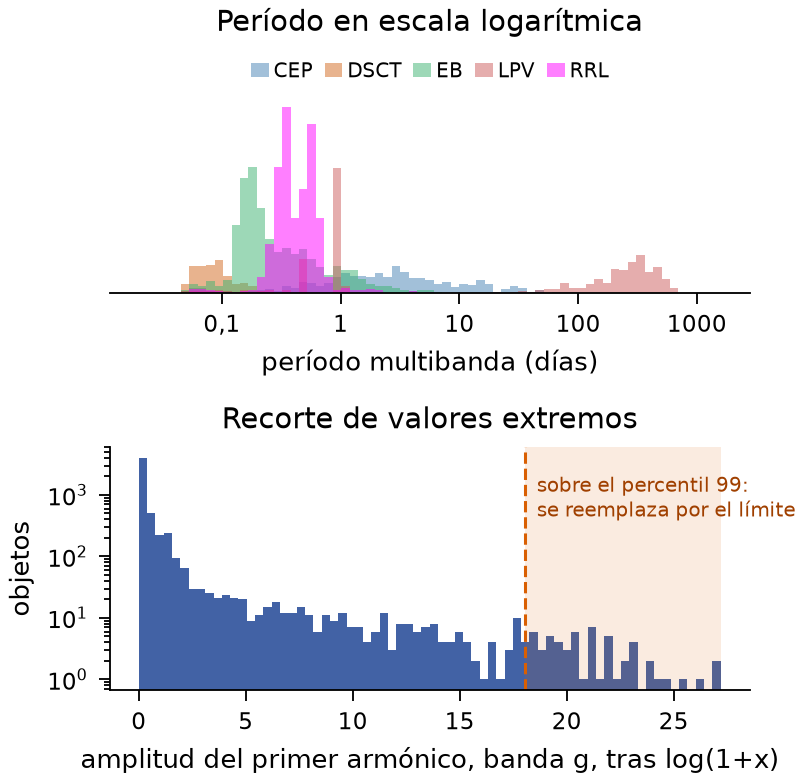
\includegraphics[width=0.96\textwidth]{figures/transformaciones.png}
\end{column}
\end{columns}
\end{frame}

% ============================================================
\begin{frame}
\frametitle{Decisión 2: normalización con z-score}
\vspace{-0.7em}
\begin{center}
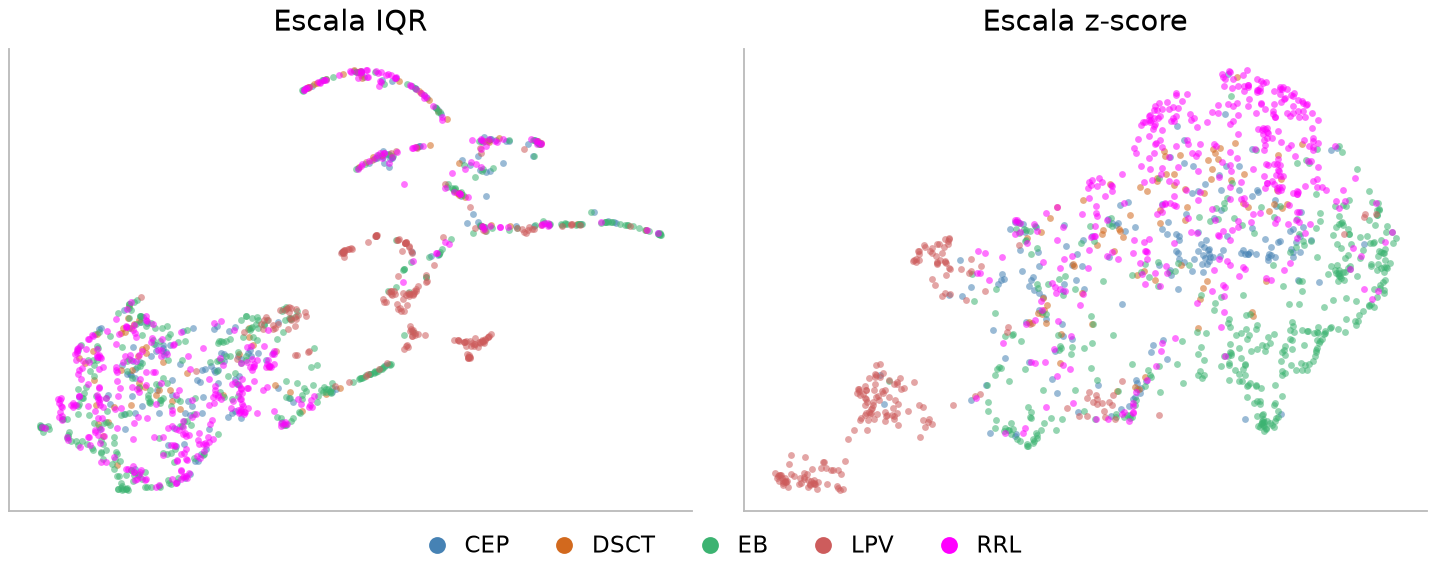
\includegraphics[width=0.63\textwidth]{figures/escala_latente.png}\\[-0.1em]
{\scriptsize Espacio latente del autoencoder en test, proyectado con UMAP
(\texttt{n\_neighbors} = 20) y coloreado por clase}
\end{center}
\vspace{-0.6em}
\begin{columns}[T]
\begin{column}{0.52\textwidth}
{\footnotesize
\begin{itemize}\itemsep=2pt
\item \textbf{Escala inicial}: mediana e IQR. En features de cola pesada quedan valores de
  hasta 300 y el autoencoder aprende esas, no el período
\item \textbf{Cambio}: z-score con media y desviación de train. Todas pesan lo mismo en el error
\end{itemize}
}
\end{column}

\begin{column}{0.45\textwidth}
\centering
{\footnotesize
\begin{tabular}{lcc}
\toprule
ARI en test & IQR & z-score \\
\midrule
Grupos del GMM      & 0,11 & \textbf{0,20} \\
Centros de MCDSVDD  & 0,36 & \textbf{0,69} \\
\bottomrule
\end{tabular}\\[0.3em]
}
\parbox{0.95\linewidth}{\centering\scriptsize \textbf{ARI}: cuánto coinciden los grupos del
modelo con las clases reales. 0 es azar y 1 es coincidencia perfecta}
\end{column}
\end{columns}
\end{frame}

% ============================================================
\begin{frame}
\frametitle{Metodología: del dato al cluster}
\vspace{-0.6em}
\begin{center}
\begin{tikzpicture}[
  stage/.style={draw=black, thick, rounded corners=1pt, align=center,
                execute at begin node={\hyphenpenalty=10000},
                text width=2.25cm, minimum height=0.95cm, font=\scriptsize, inner sep=3pt},
  modelo/.style={draw=structure, thick, rounded corners=1pt, align=center, text=structure,
                execute at begin node={\hyphenpenalty=10000},
                text width=2.55cm, minimum height=0.72cm, font=\scriptsize, inner sep=3pt},
  fl/.style={->, >=stealth, thick}]

  \node[stage] (d)                     {158 features\\ por estrella};
  \node[stage, right=0.30cm of d] (p)  {preprocesamiento\\ ajustado en train};
  \node[stage, right=0.30cm of p] (a)  {autoencoder\\ 512--256--128--\textbf{8}};
  \node[modelo, right=0.45cm of a, yshift=0.50cm]  (g) {GMM\\ sin etiquetas};
  \node[modelo, right=0.45cm of a, yshift=-0.50cm] (m) {MCDSVDD\\ con etiquetas};
  \node[stage, right=3.45cm of a] (c)  {curvas de luz:\\ prototipos y outliers};

  \draw[fl] (d) -- (p);
  \draw[fl] (p) -- (a);
  \draw[fl] (a.east) -- (g.west);
  \draw[fl] (a.east) -- (m.west);
  \draw[fl] (g.east) -- (c.west);
  \draw[fl] (m.east) -- (c.west);
\end{tikzpicture}
\end{center}
\vspace{-0.4em}
\begin{columns}[T]
\begin{column}{0.50\textwidth}
{\footnotesize
\begin{itemize}\itemsep=3pt
\item \textbf{Partición} 70/15/15 estratificada. Recorte, imputación y escala se ajustan solo
  con train: sin fuga de información
\item \textbf{Autoencoder}: MLP con BatchNorm y LeakyReLU, salida lineal, error cuadrático
  medio, Adam y \emph{early stopping} con validación
\item \textbf{Herramientas}: Python, PyTorch, scikit-learn y umap-learn. Código con pruebas
  en GitHub
\end{itemize}
}
\end{column}

\begin{column}{0.47\textwidth}
\centering
{\footnotesize \textbf{Decisión 3: tamaño del cuello de botella}}\\[0.25em]
{\scriptsize \setlength{\tabcolsep}{3pt}
\begin{tabular}{cccc}
\toprule
Dimensión & Error (MSE) & ARI GMM & ARI MCDSVDD \\
\midrule
2  & 0,54 & 0,13 & 0,55 \\
4  & 0,42 & 0,20 & 0,77 \\
\textbf{8} & 0,34 & 0,21 & \textbf{0,80} \\
16 & 0,26 & 0,23 & 0,79 \\
32 & 0,21 & 0,33 & 0,78 \\
\bottomrule
\end{tabular}\\[0.4em]
\parbox{0.97\linewidth}{\centering\scriptsize \textbf{ARI}: coincidencia de los grupos con las
clases reales (0 es azar, 1 es perfecta), en validación y promediando 3 semillas. Con menos de
8 se pierde información y 8 es el máximo de MCDSVDD}
}
\end{column}
\end{columns}
\end{frame}


% ---------- 3. Resultados preliminares ----------
% ============================================================
% Seccion: Resultados preliminares
% Etapa 3 (GMM y MCDSVDD) y etapa 4 (curvas de luz y outliers)
% Todas las metricas son del conjunto de test
% Figuras: figures/gmm.png, mcdsvdd.png, prototipos.png, outliers.png
% ============================================================
\section{Resultados preliminares}

% ============================================================
\begin{frame}
\frametitle{Etapa 3: clustering con mezcla de gaussianas (GMM)}
\vspace{-0.8em}
\begin{center}
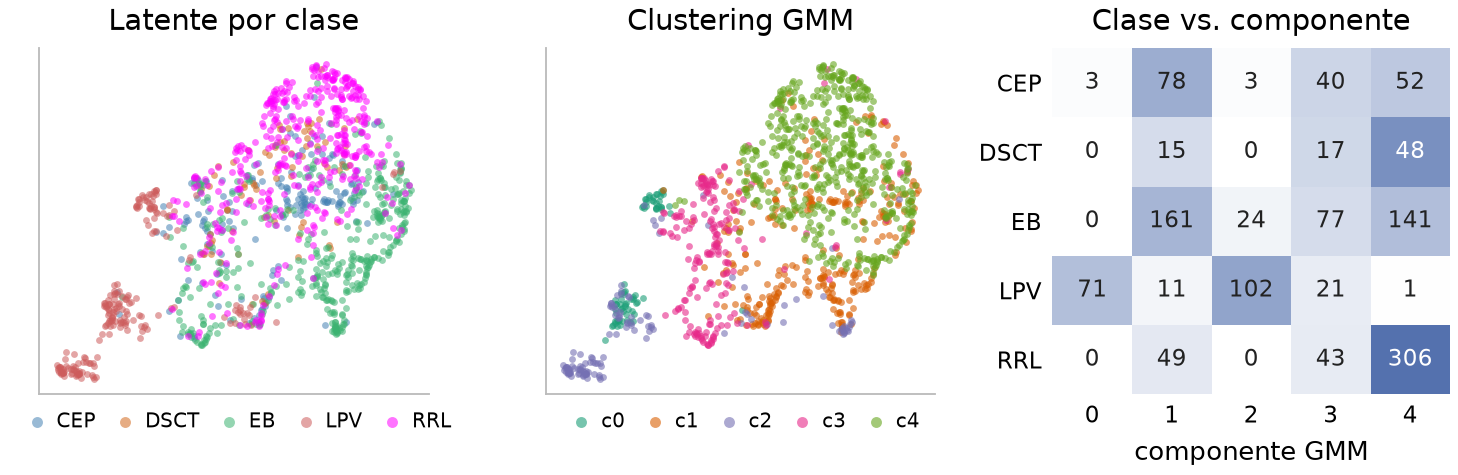
\includegraphics[width=0.78\textwidth]{figures/gmm.png}\\[-0.2em]
{\scriptsize UMAP del latente en test (\texttt{n\_neighbors} = 20). El GMM agrupa en las 8
dimensiones, no sobre el UMAP}
\end{center}
\vspace{-0.7em}
\begin{columns}[T]
\begin{column}{0.50\textwidth}
{\footnotesize \textbf{Decisiones}
\begin{itemize}\itemsep=2pt
\item 5 componentes, uno por clase, para comparar con las etiquetas (el BIC prefiere 10)
\item Covarianza completa. Se ajusta solo con el latente de train y sin etiquetas, que solo
  sirven para medir
\end{itemize}
}
\end{column}

\begin{column}{0.47\textwidth}
{\footnotesize \textbf{Resultado en test}: \textcolor{structure}{\textbf{ARI 0,20 \quad NMI 0,26}}
\begin{itemize}\itemsep=2pt
\item Recupera LPV: 173 de 206 caen en dos componentes casi puros
\item CEP, DSCT, EB y RRL quedan mezcladas: sin etiquetas, el latente no las separa
\end{itemize}
}
\end{column}
\end{columns}
\end{frame}

% ============================================================
\begin{frame}
\frametitle{Etapa 3: clustering con Multi-Class Deep SVDD}
\vspace{-0.8em}
\begin{center}
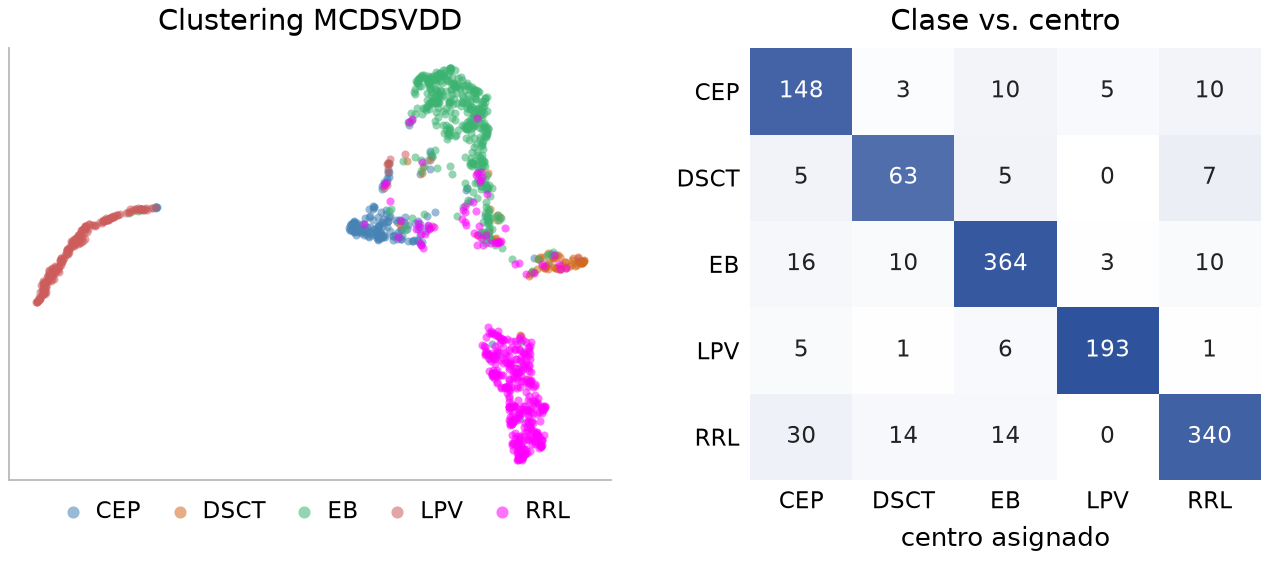
\includegraphics[width=0.66\textwidth]{figures/mcdsvdd.png}\\[-0.2em]
{\scriptsize UMAP del latente de MCDSVDD en test (\texttt{n\_neighbors} = 20)}
\end{center}
\vspace{-0.8em}
\begin{columns}[T]
\begin{column}{0.50\textwidth}
{\footnotesize \textbf{Decisiones}
\begin{itemize}\itemsep=1pt
\item Parte del encoder ya entrenado. Cada clase tiene un centro fijo y la pérdida es la
  distancia a él
\item Tasa $10^{-4}$ y 25 épocas, aún sin ajuste fino
\item \textbf{Sobremuestreo} de las clases chicas, solo en train
\end{itemize}
}
\end{column}

\begin{column}{0.47\textwidth}
{\footnotesize \textbf{Resultado en test}: \textcolor{structure}{\textbf{ARI 0,73 \quad NMI 0,67}}
\begin{itemize}\itemsep=2pt
\item Las cinco clases quedan mayormente en su centro
\item El sobremuestreo sube el ARI de 0,69 a 0,73, y DSCT pasa de 26 a 63 de 80 objetos en su
  centro
\end{itemize}
}
\end{column}
\end{columns}
\end{frame}

% ============================================================
\begin{frame}
\frametitle{Etapa 4: curvas de luz de los prototipos}
\vspace{-0.8em}
\begin{center}
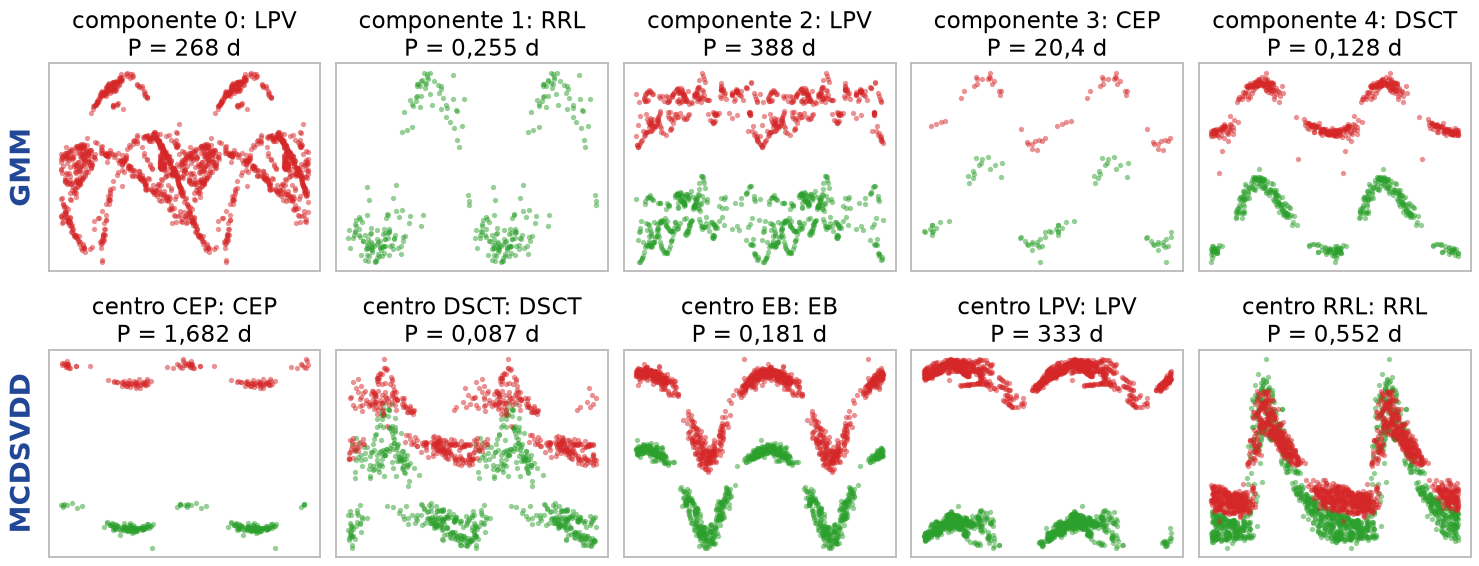
\includegraphics[width=0.93\textwidth]{figures/prototipos.png}\\[-0.1em]
{\scriptsize Prototipo: el objeto de test más cercano al centro de cada grupo. Curvas plegadas
con el período multibanda}
\end{center}
\vspace{-0.5em}
{\footnotesize
\begin{itemize}\itemsep=2pt
\item \textbf{GMM}: los componentes 0 y 2 agrupan estrellas LPV. Los componentes 1, 3 y 4
  mezclan varias clases de período corto, y por eso su prototipo puede ser de cualquiera de ellas
\item \textbf{MCDSVDD}: cada centro muestra la curva típica de su clase
\end{itemize}
}
\end{frame}

% ============================================================
\begin{frame}
\frametitle{Etapa 4: análisis de outliers}
\vspace{-0.8em}
\begin{center}
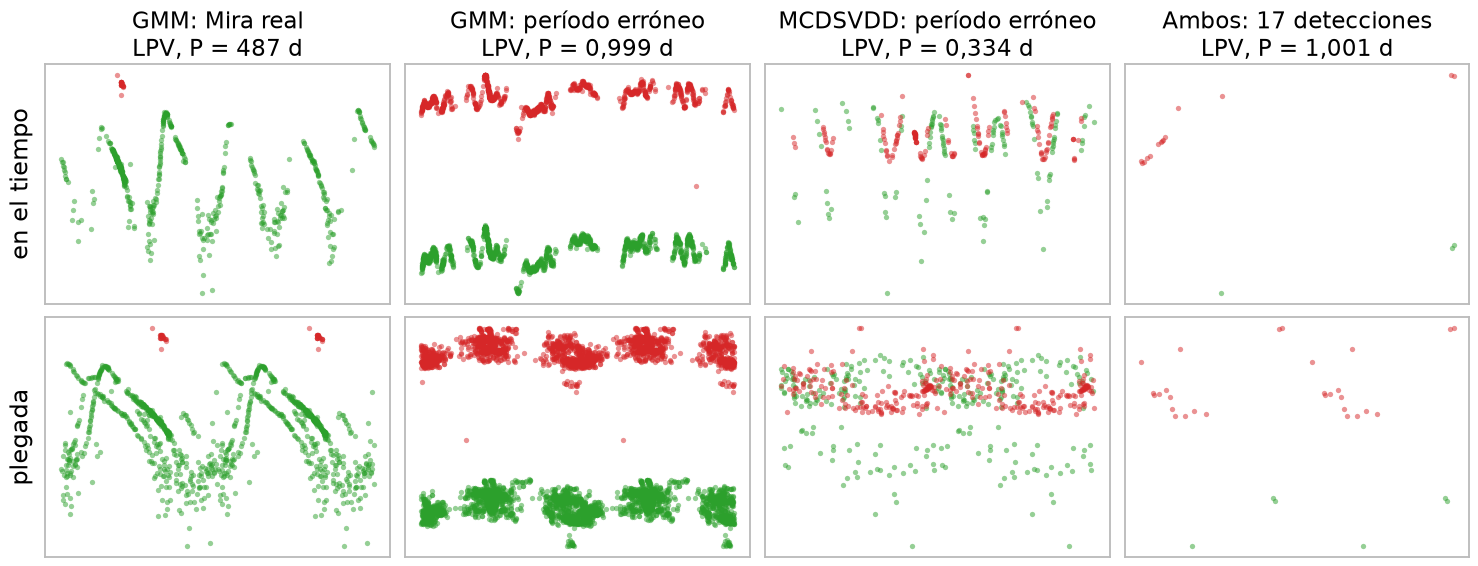
\includegraphics[width=0.90\textwidth]{figures/outliers.png}
\end{center}
\vspace{-0.6em}
{\footnotesize
\begin{itemize}\itemsep=2pt
\item \textbf{GMM} (menor verosimilitud): 5 de los 6 más extremos son LPV. Hay Miras reales de
  gran amplitud y otras con el período mal calculado
\item \textbf{MCDSVDD} (mayor distancia a los centros): objetos con pocas detecciones o con el
  período mal calculado
\item \textbf{Hallazgo}: varios outliers no son estrellas raras, sino objetos con datos malos
\end{itemize}
}
\end{frame}


% ---------- 4. Plan de trabajo hasta el final del semestre ----------
% ============================================================
% Seccion: Plan de trabajo hasta el final del semestre
% Los porcentajes de avance son una estimacion del grupo: ajustarlos aqui
% ============================================================
\section{Plan de trabajo}

% ============================================================
\begin{frame}
\frametitle{Estado de avance y plan de trabajo}
\vspace{-0.5em}
\begin{columns}[T]
\begin{column}{0.42\textwidth}
{\small \textbf{Avance por etapa}}
\vspace{0.5em}

\begin{tikzpicture}[x=1cm, y=1cm]
  \foreach \y/\nombre/\p in {%
      0/{1. Exploración de los datos}/100,
      -1.0/{2. Visualización con autoencoder}/90,
      -2.0/{3. Clustering: GMM y MCDSVDD}/80,
      -3.0/{4. Curvas de luz y outliers}/60}{
    \node[font=\footnotesize, anchor=west, inner sep=0pt] at (0,\y+0.32) {\nombre};
    \fill[structure!18, rounded corners=1pt] (0,\y-0.12) rectangle (4.4,\y+0.08);
    \fill[structure, rounded corners=1pt] (0,\y-0.12) rectangle ({4.4*\p/100},\y+0.08);
    \node[font=\footnotesize\bfseries, text=structure, anchor=west] at (4.5,\y-0.02) {\p\,\%};
  }
\end{tikzpicture}

\vspace{0.6em}
{\footnotesize \textbf{Resultado esperado}: un ranking de anomalías depurado de errores de datos,
evaluado con AUROC y respaldado con las curvas de luz.}
\end{column}

\begin{column}{0.55\textwidth}
{\small \textbf{Próximos pasos}}
\vspace{0.1em}
{\footnotesize
\begin{enumerate}\itemsep=3pt
\item Experimento de anomalías: ocultar una clase, reentrenar y medir si el modelo la marca
  como rara (AUROC)
\item Filtrar períodos en alias y objetos con pocas detecciones antes de calcular el puntaje
  de anomalía
\item Completar la etapa 4 en MCDSVDD: pertenencia a más de un cluster y sub-clusters (ya
  hecho para el GMM)
\item Ajustar los hiperparámetros de MCDSVDD
\end{enumerate}
}
\vspace{0.2em}
{\small \textbf{Aristas posibles}}
\vspace{0.1em}
{\footnotesize
\begin{itemize}\itemsep=2pt
\item Autoencoder solo con período y color para el GMM: en validación el ARI sube de 0,21 a
  0,33
\item Latente distinto por modelo: con 32 dimensiones el GMM también llega a 0,33
\item Entrenamiento conjunto de autoencoder y GMM, como en DAGMM
\end{itemize}
}
\end{column}
\end{columns}
\end{frame}


\end{document}
